% AdaPres -- IRIS 2027 (Springer LNEE) draft.
% Every result number in this file is a macro from numbers.tex (generated by make_numbers.py from results/).
% Do not type result numbers by hand. Configuration constants (5 fps, 640 px, T4, 10 seeds) are not results.
%
% Class: uses Springer's svproc.cls when present (put svproc.cls next to this file, from the IRIS/Springer
% author kit [VERIFY which class IRIS requires]); otherwise falls back to an LNCS-sized article layout so the
% draft still compiles and the page count is approximately right.
\newif\ifspringer
\IfFileExists{svproc.cls}{\springertrue}{\springerfalse}
\ifspringer
  \documentclass{svproc}
\else
  \documentclass[10pt]{article}
  \usepackage[paperwidth=155mm,paperheight=235mm,textwidth=122mm,textheight=193mm,centering]{geometry}
  \usepackage{mathptmx}
  \newcommand{\inst}[1]{\textsuperscript{#1}}
  \newcommand{\email}[1]{\texttt{#1}}
  \newcommand{\institute}[1]{}
  \providecommand{\and}{\quad}
  \newenvironment{keywords}{\par\noindent\small\raggedright\textbf{Keywords:}~\def\and{\unskip,~}}{\par}
  \renewenvironment{abstract}{\small\quotation\noindent\textbf{Abstract.}~}{\endquotation}
\fi
\usepackage[T1]{fontenc}
\usepackage[utf8]{inputenc}
\usepackage{amsmath,amssymb}
\usepackage{graphicx}
\usepackage{booktabs}
\usepackage{microtype}
\usepackage{xcolor}
\usepackage[hidelinks]{hyperref}
\usepackage{url}
\graphicspath{{figs/}}
% generated by paper/make_numbers.py from results/ -- do not edit
% results commit 4e35b3e1d68453b5e17eb15c09293e3d94eaabe3
\newcommand{\BootResamples}{1{,}000}
\newcommand{\CalibClips}{20}
\newcommand{\CalibConfigs}{32{,}376}
\newcommand{\CalibDropMain}{0.44}
\newcommand{\CommitRun}{4e35b3e1}
\newcommand{\CueCostMs}{2.70}
\newcommand{\DeltaPts}{0.5}
\newcommand{\DiffAdaptiveFPsixteenCIHi}{-0.13}
\newcommand{\DiffAdaptiveFPsixteenCILo}{-2.42}
\newcommand{\DiffAdaptiveFPsixteenMean}{-1.00}
\newcommand{\DiffAdaptiveINTeightCIHi}{+0.27}
\newcommand{\DiffAdaptiveINTeightCILo}{-0.53}
\newcommand{\DiffAdaptiveINTeightMean}{+0.03}
\newcommand{\DiffAdaptiveRandomIidCIHi}{+0.21}
\newcommand{\DiffAdaptiveRandomIidCILo}{-1.38}
\newcommand{\DiffAdaptiveRandomIidMean}{-0.38}
\newcommand{\DiffAdaptiveRandomMatchedCIHi}{+0.27}
\newcommand{\DiffAdaptiveRandomMatchedCILo}{-0.70}
\newcommand{\DiffAdaptiveRandomMatchedMean}{+0.01}
\newcommand{\DiffOracleFPsixteenCIHi}{+0.48}
\newcommand{\DiffOracleFPsixteenCILo}{-0.55}
\newcommand{\DiffOracleFPsixteenMean}{-0.10}
\newcommand{\DriftFPsixteen}{0.08}
\newcommand{\DriftINTeight}{0.21}
\newcommand{\DropAdaptiveVsFPsixteen}{0.90}
\newcommand{\DropINTeightVsFPsixteen}{0.94}
\newcommand{\EDynAdaptPipe}{178}
\newcommand{\EDynAdaptSeq}{79}
\newcommand{\EDynFPsixteen}{204}
\newcommand{\EDynFPthirtytwo}{365}
\newcommand{\EDynINTeight}{167}
\newcommand{\ETotalAdaptPipe}{363}
\newcommand{\ETotalAdaptSeq}{369}
\newcommand{\ETotalFPsixteen}{393}
\newcommand{\ETotalFPthirtytwo}{723}
\newcommand{\ETotalINTeight}{333}
\newcommand{\EngineMsFPsixteen}{2.70}
\newcommand{\EngineMsFPthirtytwo}{7.78}
\newcommand{\EngineMsINTeight}{1.99}
\newcommand{\EngineSpeedupINTeightPct}{26}
\newcommand{\FpsAdaptPipe}{175}
\newcommand{\FpsAdaptSeq}{112}
\newcommand{\FpsFPsixteen}{172}
\newcommand{\FpsFPthirtytwo}{91}
\newcommand{\FpsINTeight}{197}
\newcommand{\FracINTeightAdaptive}{0.96}
\newcommand{\FracINTeightFixedFPsixteen}{0.00}
\newcommand{\FracINTeightFixedFPthirtytwo}{0.00}
\newcommand{\FracINTeightFixedINTeight}{1.00}
\newcommand{\FracINTeightOracle}{0.63}
\newcommand{\FracINTeightRandomIid}{0.50}
\newcommand{\FracINTeightRandomMatched}{0.96}
\newcommand{\HFourEasyShare}{0.505}
\newcommand{\HFourResult}{supported}
\newcommand{\HOneResult}{not supported}
\newcommand{\HThreeResult}{supported}
\newcommand{\HTwoResult}{not supported}
\newcommand{\LatAdaptPipe}{5.54}
\newcommand{\LatAdaptSeq}{8.85}
\newcommand{\LatFPsixteen}{5.78}
\newcommand{\LatFPthirtytwo}{11.02}
\newcommand{\LatINTeight}{5.03}
\newcommand{\LatPninetyfiveAdaptPipe}{6.57}
\newcommand{\LatPninetyfiveAdaptSeq}{9.50}
\newcommand{\LatPninetyfiveFPsixteen}{6.07}
\newcommand{\LatPninetyfiveFPthirtytwo}{11.44}
\newcommand{\LatPninetyfiveINTeight}{5.34}
\newcommand{\LiveAgreementPct}{100}
\newcommand{\LiveFrames}{1{,}924}
\newcommand{\MapAdaptive}{25.81}
\newcommand{\MapAdaptiveCIHi}{36.06}
\newcommand{\MapAdaptiveCILo}{22.18}
\newcommand{\MapAdaptiveCrowded}{23.82}
\newcommand{\MapAdaptiveEasy}{33.91}
\newcommand{\MapAdaptiveNight}{11.64}
\newcommand{\MapAdaptiveSceneChange}{20.65}
\newcommand{\MapChangeKEight}{+0.14}
\newcommand{\MapChangeKFive}{+0.02}
\newcommand{\MapChangeKThree}{-0.00}
\newcommand{\MapChangeKTwo}{+0.00}
\newcommand{\MapFiftyAdaptive}{41.23}
\newcommand{\MapFiftyFixedFPsixteen}{42.95}
\newcommand{\MapFiftyFixedFPthirtytwo}{42.95}
\newcommand{\MapFiftyFixedINTeight}{41.27}
\newcommand{\MapFiftyOracle}{43.28}
\newcommand{\MapFiftyRandomIid}{42.04}
\newcommand{\MapFiftyRandomMatched}{41.26}
\newcommand{\MapFixedFPsixteen}{26.71}
\newcommand{\MapFixedFPsixteenCIHi}{36.93}
\newcommand{\MapFixedFPsixteenCILo}{22.99}
\newcommand{\MapFixedFPsixteenCrowded}{24.50}
\newcommand{\MapFixedFPsixteenEasy}{34.01}
\newcommand{\MapFixedFPsixteenNight}{12.55}
\newcommand{\MapFixedFPsixteenSceneChange}{21.61}
\newcommand{\MapFixedFPthirtytwo}{26.70}
\newcommand{\MapFixedFPthirtytwoCIHi}{36.93}
\newcommand{\MapFixedFPthirtytwoCILo}{22.99}
\newcommand{\MapFixedFPthirtytwoCrowded}{24.50}
\newcommand{\MapFixedFPthirtytwoEasy}{33.98}
\newcommand{\MapFixedFPthirtytwoNight}{12.59}
\newcommand{\MapFixedFPthirtytwoSceneChange}{21.80}
\newcommand{\MapFixedINTeight}{25.76}
\newcommand{\MapFixedINTeightCIHi}{36.10}
\newcommand{\MapFixedINTeightCILo}{22.08}
\newcommand{\MapFixedINTeightCrowded}{23.53}
\newcommand{\MapFixedINTeightEasy}{33.91}
\newcommand{\MapFixedINTeightNight}{11.61}
\newcommand{\MapFixedINTeightSceneChange}{18.68}
\newcommand{\MapOracle}{26.67}
\newcommand{\MapOracleCIHi}{37.09}
\newcommand{\MapOracleCILo}{22.92}
\newcommand{\MapOracleCrowded}{24.34}
\newcommand{\MapOracleEasy}{34.24}
\newcommand{\MapOracleNight}{12.31}
\newcommand{\MapOracleSceneChange}{21.56}
\newcommand{\MapRandomIid}{26.16}
\newcommand{\MapRandomIidCIHi}{36.40}
\newcommand{\MapRandomIidCILo}{22.46}
\newcommand{\MapRandomIidCrowded}{23.95}
\newcommand{\MapRandomIidEasy}{33.84}
\newcommand{\MapRandomIidNight}{12.05}
\newcommand{\MapRandomIidSD}{0.11}
\newcommand{\MapRandomIidSceneChange}{20.33}
\newcommand{\MapRandomMatched}{25.77}
\newcommand{\MapRandomMatchedCIHi}{36.12}
\newcommand{\MapRandomMatchedCILo}{22.08}
\newcommand{\MapRandomMatchedCrowded}{23.55}
\newcommand{\MapRandomMatchedEasy}{33.85}
\newcommand{\MapRandomMatchedNight}{11.63}
\newcommand{\MapRandomMatchedSD}{0.06}
\newcommand{\MapRandomMatchedSceneChange}{18.91}
\newcommand{\SceneChangeFrames}{160}
\newcommand{\SwitchPenaltyMs}{-0.08}
\newcommand{\SwitchRateAdaptive}{1.48}
\newcommand{\SwitchRateFixedFPsixteen}{0.00}
\newcommand{\SwitchRateFixedFPthirtytwo}{0.00}
\newcommand{\SwitchRateFixedINTeight}{0.00}
\newcommand{\SwitchRateKEight}{1.03}
\newcommand{\SwitchRateKFive}{1.18}
\newcommand{\SwitchRateKOne}{1.48}
\newcommand{\SwitchRateKThree}{1.21}
\newcommand{\SwitchRateKTwo}{1.30}
\newcommand{\SwitchRateOracle}{34.08}
\newcommand{\SwitchRateRandomIid}{50.13}
\newcommand{\SwitchRateRandomMatched}{1.45}
\newcommand{\TestClips}{40}
\newcommand{\TestFrames}{7{,}796}


% ---- review markers (remove before submission) --------------------------------------------
\newcommand{\VERIFY}[1]{\textcolor{red}{[VERIFY: #1]}}
\newcommand{\TODO}[1]{\textcolor{red}{[TODO: #1]}}

\begin{document}

% DECISION FOR THE AUTHORS: the registered title promises hardware awareness and Jetson/VisDrone results.
% The hardware (contention) term was implemented but not evaluated (w_h = 0), and neither VisDrone nor Jetson was run.
% Proposed honest title below; the registered title is kept commented out.
\title{Content-Aware Adaptive Precision for Real-Time Video Object Detection: An Oracle-Referenced Evaluation}
% \title{Content- and Hardware-Aware Adaptive Precision for Real-Time Video Object Detection}
\author{
  Vinay Kamble\inst{1} \and
  Aisshwarya Gurav\inst{1} \and
  Shrejal Bhosale\inst{1} \and
  Dr. Uma Gurav\inst{1}
}

\ifspringer
  \institute{
    Department of Computer Science and Engineering
    (Artificial Intelligence and Machine Learning),\\
    KIT's College of Engineering, Kolhapur,
    Maharashtra, India\\
    \email{
      vinaykamble289@gmail.com,
      aisshwaryagurav@gmail.com,
      bhosaleshrejal@gmail.com
    }\\
    \textit{Faculty Guide: Dr. Uma Gurav,
    Head of Department, CSE (AI \& ML)}
  }
  \maketitle
\else
  \date{}
  \maketitle
  \vspace{-2em}
  \begin{center}
    \small
    Department of Computer Science and Engineering
    (Artificial Intelligence and Machine Learning)\\
    KIT's College of Engineering, Kolhapur,
    Maharashtra, India\\[4pt]
    \texttt{vinaykamble289@gmail.com}\\
    \texttt{aisshwaryagurav@gmail.com}\\
    \texttt{bhosaleshrejal@gmail.com}\\[4pt]
    \textit{Faculty Guide: Dr. Uma Gurav}\\
    \textit{Head of Department, CSE (AI \& ML)}
  \end{center}
\fi

\begin{abstract}
Real-time video detectors are usually deployed at one fixed numerical precision, even though some frames
may tolerate lower precision than others. We study whether a lightweight, content-aware controller can exploit
this by choosing, per frame, between INT8 and FP16 TensorRT engines of a COCO-pretrained YOLO11s detector. The controller scores frame difficulty from
frame-difference motion, edge-density clutter, the previous frame's detection count and confidence, and a
histogram scene-change cue, and switches only after the decision has persisted for $K$ frames. All thresholds and weights are calibrated on held-out clips and locked before testing, and the hypotheses were pre-registered.
On \TestClips{} BDD100K tracking clips (\TestFrames{} frames, one Tesla T4 GPU), an oracle that picks the
cheapest adequate engine per frame matches FP16 accuracy (\MapOracle{} vs.\ \MapFixedFPsixteen{} mAP@0.5:0.95)
while using INT8 on \FracINTeightOracle{} of frames, so per-frame headroom exists. The locked controller does not capture it: it
runs INT8 on \FracINTeightAdaptive{} of frames and is statistically indistinguishable from fixed INT8 and from
random switching with the same precision mix (\MapAdaptive{} vs.\ \MapFixedINTeight{} and \MapRandomMatched{}).
We trace the failure to the instability of slice-level INT8 sensitivity: at night, INT8 was
$\GapCalibNight$ points better than FP16 on the calibration clips but $\GapTestNight$ points worse on the test clips. Measured on the GPU, adaptive execution also
costs more energy per frame than fixed INT8 (\ETotalAdaptPipe{} vs.\ \ETotalINTeight{} mJ). We release the
evaluation protocol, including the oracle, matched-random baseline and replay-versus-live validation, as a template for testing adaptive-inference claims.
\end{abstract}
\begin{keywords}
Real-time object detection \and Video analytics \and Quantization \and Adaptive inference \and YOLO \and Negative result
\end{keywords}

% ============================================================================================
\section{Introduction}
Object detection on video streams underpins driver assistance, traffic monitoring and aerial surveillance,
where accuracy must be traded against latency and energy. Post-training quantization to INT8 reduces inference
cost with modest accuracy loss for many convolutional networks~\cite{jacob2018,nagel2021}, but a deployment
normally fixes one precision for every frame. Intuitively, an empty daytime road should tolerate INT8, while a crowded
intersection at night may need FP16. Instance-adaptive quantization~\cite{liu2022} and adaptive video-analytics
systems~\cite{chameleon2018,adascale2019,approxdet2020} have shown that input-dependent configuration choices can pay
off. This raises a simple, practical question: \emph{can cheap, hand-crafted content cues decide per frame when INT8 is
good enough for an off-the-shelf detector?}

We answer this question with a deliberately conservative protocol. The controller's weights and thresholds are calibrated on held-out clips,
then locked and hashed before any test run. The hypotheses, effect sizes and model-selection rules were frozen
in advance, and every later deviation is logged. Beyond fixed-precision baselines, we compare against (i) a per-frame
oracle that uses ground truth, which bounds what any controller could achieve, and (ii) a \emph{matched-random}
baseline, which uses the controller's own precision mix and switch rate but places the switches at random. The second
comparison isolates whether the controller's \emph{choices} carry information, which a comparison against fixed
precisions alone cannot show.

\paragraph{Contributions.}
(1)~A content-aware precision controller for TensorRT YOLO engines with persistence-based switching and a
scene-change override (Sect.~\ref{sec:method}).
(2)~An oracle- and matched-random-referenced evaluation protocol with sequence-level bootstrap intervals, measured
GPU energy, and replay-versus-live validation (Sect.~\ref{sec:setup}).
(3)~Evidence on BDD100K~\cite{bdd100k} that per-frame precision headroom exists (the oracle), but that the locked
content-aware controller does not exploit it and costs more energy than fixed INT8 (Sect.~\ref{sec:results}).
(4)~A diagnosis: the accuracy cost of INT8 on a given condition (night, crowded, easy) changes sign or size
between disjoint clip sets, so mappings from content to precision calibrated on small clip sets do not transfer.

% ============================================================================================
\section{Related Work}
\paragraph{Quantization.} Integer-arithmetic inference with quantized weights and activations~\cite{jacob2018} and
post-training quantization pipelines~\cite{nagel2021} typically keep 8-bit accuracy close to floating point; we use
TensorRT's calibrated INT8 path as provided by the Ultralytics export~\cite{ultralytics}.
\paragraph{Input-adaptive quantization.} Liu et al.~\cite{liu2022} train a bit-controller jointly with the network so
that simple images receive fewer bits. This requires training and bit-width-flexible kernels. We instead study a
training-free controller that switches between two off-the-shelf engines.
\paragraph{Adaptive video analytics.} Chameleon~\cite{chameleon2018} periodically re-profiles pipeline
configurations and exploits their temporal correlation. AdaScale~\cite{adascale2019} picks the input scale per frame. ApproxDet~\cite{approxdet2020} selects among execution branches using content and resource contention. These systems adapt resolution, frame rate or branch, and report gains against fixed
configurations. We adapt numerical precision, and we add an oracle and a matched-random control. The latter is the comparison
that decides whether the adaptation policy is informative at all.

% ============================================================================================
\section{Method}\label{sec:method}
\paragraph{Engines.} A COCO-pretrained~\cite{coco} YOLO11s detector~\cite{ultralytics} (Ultralytics~8.4.216, TensorRT~10.16) is exported to TensorRT engines at FP32,
FP16 and INT8 (640\,px, batch 1). INT8 is calibrated on calibration-split frames only. The engines needed by the
controller (INT8 and FP16) stay resident, so a switch is just a choice of engine.

\paragraph{Cues.} For frame $t$ we compute, on a 320-pixel-wide grayscale copy: motion $m_t$, the mean absolute
difference to frame $t{-}1$; clutter $c_t$, the fraction of Canny edge pixels; and $d_t$, the Bhattacharyya distance
between the hue--saturation histograms of frames $t$ and $t{-}1$, giving a binary scene-change cue
$s_t=\mathbb{1}[d_t\ge\theta_{sc}]$. From the detections that the \emph{chosen} engine produced at $t{-}1$ (confidence
$\ge 0.25$) we take the count $n_t$ and uncertainty $u_t = 1-\bar{p}$, where $\bar{p}$ is their mean confidence.
Continuous cues are normalised with calibration-split percentiles, $\tilde{x}=\mathrm{clip}\big((x-p_5)/(p_{95}-p_5),0,1\big)$.

\paragraph{Score and decision.} The difficulty score is
\begin{equation}
S_t = w_m\tilde m_t + w_c\tilde c_t + w_n\tilde n_t + w_u\tilde u_t + w_s s_t,\qquad \textstyle\sum w = 1,\; w\ge 0,
\end{equation}
optionally smoothed by an exponential moving average, $\hat S_t=\alpha S_t+(1-\alpha)\hat S_{t-1}$. The controller proposes INT8 if
$\hat S_t<\theta$ and FP16 otherwise. \emph{Persistence:} a proposal that differs from the current level must repeat for $K$
consecutive frames before the controller switches (separate $K_{\uparrow}$ and $K_{\downarrow}$ are supported).
\emph{Override:} if $s_t=1$, the controller switches to FP16 immediately and holds it for $H$ frames. A hardware term
$\hat S_t - w_h h_t$, where $h_t$ is the slowdown of observed relative to isolated latency, is implemented. It is disabled
($w_h=0$) in all experiments reported here, because we could not evaluate it under controlled contention (Sect.~\ref{sec:threats}).

\paragraph{Calibration and locking.} On the calibration split only, a grid search over weights, $\theta$ (as a quantile of the
open-loop score), $K$, $\alpha$ and $\theta_{sc}$ (\CalibConfigs{} configurations) maximises the estimated latency saving
over FP16, subject to $\text{mAP@0.5:0.95}\ge \text{mAP}_\text{FP16}-\delta$ with $\delta=\DeltaPts$ points. A per-frame F1 proxy
ranks the configurations, and the top 20 are rescored with full mAP. The selected configuration is written to disk and
hashed. Test runs refuse to start unless the hash matches. The locked controller uses
$(w_m,w_c,w_n,w_u,w_s)=(\LockWm,\allowbreak\LockWc,\allowbreak\LockWn,\allowbreak\LockWu,\allowbreak\LockWs)$, $\theta=\LockTheta$, $K=\LockK$, $\alpha=\LockAlpha$,
$\theta_{sc}=\LockThetaSc$, $H=\LockH$. On calibration it lost \CalibDropMain{} points against FP16.

% ============================================================================================
\section{Experimental Setup}\label{sec:setup}
\paragraph{Data.} We use BDD100K~\cite{bdd100k} multi-object tracking clips, which have dense per-frame boxes at 5\,fps.
Because only the validation images of the tracking set were available in our environment, the calibration
(\CalibClips{} clips, \FramesCalibAll{} frames) and test (\TestClips{} clips, \TestFrames{} frames) splits are disjoint, seeded clip sets drawn from it and stratified by time of day.
COCO classes are mapped to the seven evaluated classes. Pedestrian and rider become \emph{person}, because COCO has no rider class, and
BDD's \emph{other person}, \emph{other vehicle} and \emph{trailer} boxes become crowd regions that are ignored when matching.
\paragraph{Slices.} The slice labels are objective and their thresholds were fixed on calibration. \emph{Night}: mean frame luma below an Otsu threshold.
\emph{Crowded}: at least the calibration 90th percentile of ground-truth objects per frame. \emph{Easy}: neither night nor
crowded, at most the median object count, and not a scene change. \emph{Scene change}: the first five frames after a splice point in 20 streams
built by concatenating test segments. This slice is synthetic (\SceneChangeFrames{} frames).
\paragraph{Baselines.} Fixed FP32, FP16 and INT8 engines; i.i.d.\ random switching (50/50); \emph{matched random}, a
two-state Markov chain whose transition matrix is estimated from the controller's own test-split decisions, so that the precision mix and switch
rate match and only the placement of switches differs (10 seeds); and \emph{oracle-cheap}, which per frame picks the cheaper engine whose
F1@0.5 is at least FP16's. The oracle uses ground truth and is not deployable.
\paragraph{Metrics.} We report mAP@0.5:0.95 and mAP@0.5 from pycocotools, read from the precision array with a maximum of 300
detections. 95\% intervals come from a cluster bootstrap over clips (\BootResamples{} resamples, paired for differences).
\paragraph{Replay and live measurement.} Every engine runs once on every frame, and policies are replayed causally on the cached outputs.
In replay, a policy's detection cues come from the engine it chose at $t{-}1$. A live run on a subset of \LiveFrames{} test frames reproduced the replayed
decisions and mAP exactly (\LiveAgreementPct\% level agreement). Latency and energy are measured live on one Tesla T4 with
pre-decoded frames: at least 20\,s of warm-up, at least 60\,s measurement windows, three interleaved repeats, and the NVML board energy counter.
The energy metric is $E_\text{total}=\Delta E/N$. The idle-subtracted $E_\text{dyn}$ is reported as secondary because it
rewards configurations that leave the GPU idle (Sect.~\ref{sec:cost}). The controller's image cues run either
\emph{sequentially} before each inference or \emph{pipelined}, with a CPU worker computing frame $t{+}1$'s cues while the GPU runs frame $t$.

% ============================================================================================
\section{Results}\label{sec:results}

\begin{table}[t]
\centering
\caption{Test split, mAP@0.5:0.95 in points (all frames and per slice), mAP@0.5, share of frames on INT8, switches per
100 frames, and estimated engine-only latency (microbenchmark medians weighted by the precision mix). Random rows: mean of 10 seeds.
$^\dagger$Synthetic (spliced) scene changes. $^\ddagger$Uses ground truth; not deployable.}
\label{tab:main}
\scriptsize\setlength{\tabcolsep}{3pt}
\begin{tabular}{@{}lrrrrrrrrr@{}}
\toprule
Policy & mAP & mAP50 & easy & crowd. & night & scene$^\dagger$ & INT8 & sw./100 & eng.\,ms\\
\midrule
FP32            & \MapFixedFPthirtytwo & \MapFiftyFixedFPthirtytwo & \MapFixedFPthirtytwoEasy & \MapFixedFPthirtytwoCrowded & \MapFixedFPthirtytwoNight & \MapFixedFPthirtytwoSceneChange & \FracINTeightFixedFPthirtytwo & \SwitchRateFixedFPthirtytwo & \EngineMsFPthirtytwo\\
FP16            & \MapFixedFPsixteen & \MapFiftyFixedFPsixteen & \MapFixedFPsixteenEasy & \MapFixedFPsixteenCrowded & \MapFixedFPsixteenNight & \MapFixedFPsixteenSceneChange & \FracINTeightFixedFPsixteen & \SwitchRateFixedFPsixteen & \EngineMsFPsixteen\\
INT8            & \MapFixedINTeight & \MapFiftyFixedINTeight & \MapFixedINTeightEasy & \MapFixedINTeightCrowded & \MapFixedINTeightNight & \MapFixedINTeightSceneChange & \FracINTeightFixedINTeight & \SwitchRateFixedINTeight & \EngineMsINTeight\\
\midrule
Adaptive (locked) & \MapAdaptive & \MapFiftyAdaptive & \MapAdaptiveEasy & \MapAdaptiveCrowded & \MapAdaptiveNight & \MapAdaptiveSceneChange & \FracINTeightAdaptive & \SwitchRateAdaptive & \EngineMsAdaptive\\
Random, matched & \MapRandomMatched & \MapFiftyRandomMatched & \MapRandomMatchedEasy & \MapRandomMatchedCrowded & \MapRandomMatchedNight & \MapRandomMatchedSceneChange & \FracINTeightRandomMatched & \SwitchRateRandomMatched & \EngineMsAdaptive\\
Random, i.i.d.  & \MapRandomIid & \MapFiftyRandomIid & \MapRandomIidEasy & \MapRandomIidCrowded & \MapRandomIidNight & \MapRandomIidSceneChange & \FracINTeightRandomIid & \SwitchRateRandomIid & \EngineMsRandomIid\\
Oracle-cheap$^\ddagger$ & \MapOracle & \MapFiftyOracle & \MapOracleEasy & \MapOracleCrowded & \MapOracleNight & \MapOracleSceneChange & \FracINTeightOracle & \SwitchRateOracle & \EngineMsOracle\\
\bottomrule
\end{tabular}
\end{table}

\begin{figure}[t]
\centering
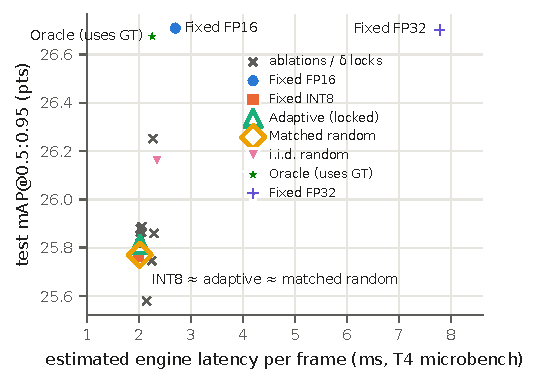
\includegraphics[width=\textwidth]{accuracy_cost}
% ALT: see figs/alt_text.json ("accuracy_cost")
\caption{Test mAP@0.5:0.95 against estimated engine-only latency (T4 microbenchmark; cue cost excluded). The dotted line
interpolates between fixed INT8 and FP16. The locked controller, the matched-random baseline and the ablations
(crosses) lie on, close to (within about 0.1 points) or below it; only the ground-truth oracle lies clearly above. FP32 (\MapFixedFPthirtytwo{} points at
\EngineMsFPthirtytwo{}\,ms) is outside the plotted range.}
\label{fig:acccost}
\end{figure}

\subsection{Is there headroom?}
FP32 and FP16 are indistinguishable (\MapFixedFPthirtytwo{} vs.\ \MapFixedFPsixteen{} points), and INT8 costs
\DropINTeightVsFPsixteen{} points while cutting engine latency by \EngineSpeedupINTeightPct\% (\EngineMsINTeight{} vs.\
\EngineMsFPsixteen{}\,ms; Table~\ref{tab:main}). The oracle keeps FP16 accuracy
(\MapOracle{} points; difference to FP16 $\DiffOracleFPsixteenMean$, 95\% CI [$\DiffOracleFPsixteenCILo$, $\DiffOracleFPsixteenCIHi$])
while running INT8 on \FracINTeightOracle{} of frames, a \EngineSavingOraclePct\% engine-latency saving. Per-frame headroom
therefore exists. Because the oracle also benefits from frame-level noise in F1, this saving is an upper bound.

\subsection{Does the controller find it?}
No. The locked controller runs INT8 on \FracINTeightAdaptive{} of test frames and reaches \MapAdaptive{} points. Relative to fixed FP16
it loses $\DiffAdaptiveFPsixteenMean$ points (CI [$\DiffAdaptiveFPsixteenCILo$, $\DiffAdaptiveFPsixteenCIHi$]), exceeding the
calibrated tolerance $\delta=\DeltaPts$ that it met on calibration (drop \CalibDropMain{}). Against fixed INT8 the difference is
$\DiffAdaptiveINTeightMean$ (CI [$\DiffAdaptiveINTeightCILo$, $\DiffAdaptiveINTeightCIHi$]). Against matched random,
the decisive comparison, it is $\DiffAdaptiveRandomMatchedMean$ (CI [$\DiffAdaptiveRandomMatchedCILo$, $\DiffAdaptiveRandomMatchedCIHi$]).
At the same precision mix and switch rate, the controller's placement of FP16 frames is no better than chance.
Fig.~\ref{fig:acccost} shows the same picture for all \emph{re-calibrated} variants: every content-aware
configuration lies on, close to or below the line interpolating between INT8 and FP16. The largest excursion above it is the uncertainty-only ablation
(\MapSU{} points at \FracINTeightSU{} INT8; exploratory, Sect.~\ref{sec:ablations}), still far below the oracle. The one slice where the controller clearly beats fixed INT8 is
the synthetic scene-change slice (\MapAdaptiveSceneChange{} vs.\ \MapFixedINTeightSceneChange{}). There the histogram cue and the override
fire at the splice points by construction (FP16 on \PctFPsixteenAdaptiveSceneChange\% of those frames), so this is not
evidence about natural content changes.

\subsection{Why does it fail?}\label{sec:why}
Table~\ref{tab:gap} compares the INT8$-$FP16 accuracy gap per slice on the two disjoint clip sets, using the same engines. The
gap is not stable. On the calibration clips, INT8 was \emph{better} than FP16 at night ($\GapCalibNight$) and much
worse on easy frames ($\GapCalibEasy$). On the test clips the night gap is $\GapTestNight$ and the easy gap only
$\GapTestEasy$. Night frames have low motion and clutter, so they score low, and calibration found nothing to correct this: the controller ran INT8 on
\PctINTeightAdaptiveNight\% of test night frames, where INT8 is now the worse choice. The calibration objective also
degenerated. The sequential cue cost (\CueCostMs\,ms per frame) is constant, so maximising the saving within $\delta$ amounts to maximising
the INT8 share, which pushed the lock to the edge of the constraint ($K=\LockK$, \FracINTeightAdaptive{} INT8). In short, with
\CalibClips{} calibration clips the per-condition sensitivity of INT8 is dominated by clip-to-clip variation, and coarse content cues
cannot predict it.

\begin{table}[t]
\centering
\caption{INT8$-$FP16 mAP@0.5:0.95 gap (points) per slice on the disjoint calibration and test clip sets (same engines),
and the locked controller's share of INT8 frames on test.}
\label{tab:gap}
\scriptsize
\begin{tabular}{@{}lrrrrr@{}}
\toprule
Slice & calib.\ frames & calib.\ gap & test frames & test gap & controller INT8 (test, \%)\\
\midrule
all     & \FramesCalibAll     & $\GapCalibAll$     & \FramesTestAll     & $\GapTestAll$     & -- \\
easy    & \FramesCalibEasy    & $\GapCalibEasy$    & \FramesTestEasy    & $\GapTestEasy$    & \PctINTeightAdaptiveEasy\\
crowded & \FramesCalibCrowded & $\GapCalibCrowded$ & \FramesTestCrowded & $\GapTestCrowded$ & \PctINTeightAdaptiveCrowded\\
night   & \FramesCalibNight   & $\GapCalibNight$   & \FramesTestNight   & $\GapTestNight$   & \PctINTeightAdaptiveNight\\
\bottomrule
\end{tabular}
\end{table}

\subsection{What does adaptivity cost?}\label{sec:cost}
Table~\ref{tab:energy} reports live measurements. With sequential cues, adaptive execution is slower than FP16
(\LatAdaptSeq{} vs.\ \LatFPsixteen\,ms median). Pipelining the image cues hides most of this (\LatAdaptPipe\,ms), but it remains
slower than fixed INT8 (\LatINTeight\,ms) and draws more energy per frame (\ETotalAdaptPipe{} vs.\ \ETotalINTeight\,mJ), even though
the controller chose INT8 on every frame of this measurement subset. Keeping both engines resident costs \MemAdaptive\,MiB of GPU memory, against \MemINTeight\,MiB
for INT8 alone. The idle-subtracted metric illustrates a measurement pitfall: the sequential controller leaves the GPU waiting
while the CPU computes cues, so subtracting idle power over the whole window makes it look cheapest ($E_\text{dyn}=\EDynAdaptSeq$\,mJ), although
it draws more total energy than INT8. We therefore report $E_\text{total}$ as the primary metric. We changed this after seeing the results; both metrics are reported in full.

\begin{table}[t]
\centering
\caption{Live measurements on one Tesla T4 (pre-decoded frames; median of three interleaved repeats). Energy is GPU board
energy from the NVML counter. Memory is the GPU memory added by the resident engine(s).}
\label{tab:energy}
\scriptsize
\begin{tabular}{@{}lrrrrrr@{}}
\toprule
Configuration & lat.\ median (ms) & p95 (ms) & FPS & $E_\text{total}$ (mJ) & $E_\text{dyn}$ (mJ) & GPU mem.\ (MiB)\\
\midrule
FP32 & \LatFPthirtytwo & \LatPninetyfiveFPthirtytwo & \FpsFPthirtytwo & \ETotalFPthirtytwo & \EDynFPthirtytwo & \MemFPthirtytwo\\
FP16 & \LatFPsixteen & \LatPninetyfiveFPsixteen & \FpsFPsixteen & \ETotalFPsixteen & \EDynFPsixteen & \MemFPsixteen\\
INT8 & \LatINTeight & \LatPninetyfiveINTeight & \FpsINTeight & \ETotalINTeight & \EDynINTeight & \MemINTeight\\
Adaptive, sequential cues & \LatAdaptSeq & \LatPninetyfiveAdaptSeq & \FpsAdaptSeq & \ETotalAdaptSeq & \EDynAdaptSeq & \MemAdaptive\\
Adaptive, pipelined cues & \LatAdaptPipe & \LatPninetyfiveAdaptPipe & \FpsAdaptPipe & \ETotalAdaptPipe & \EDynAdaptPipe & \MemAdaptive\\
\bottomrule
\end{tabular}
\end{table}

\subsection{Ablations, persistence and hypotheses}\label{sec:ablations}
Each ablation was re-calibrated and locked like the main controller (Table~\ref{tab:abl}). Removing any single cue changes test mAP
by at most a few hundredths to tenths of a point. Most variants converge on the same INT8-heavy operating point. The exception is dropping the count cue, which lowers the INT8 share to \FracAblAn{} without
improving accuracy ($\DeltaAblAn$). Among the single-cue controllers, uncertainty-only reaches \MapAblSu{} points at
\FracAblSu{} INT8, slightly above the INT8--FP16 interpolation in Fig.~\ref{fig:acccost}. We report this only as an
exploratory lead: it was not a pre-registered hypothesis and was singled out after the test results were seen. The scene-change-only
controller collapses to always-FP16. Persistence barely matters at this operating point. With $\theta$ fixed and $K$ swept,
the switch rate falls from \SwitchRateKOne{} ($K{=}1$) to \SwitchRateKEight{} ($K{=}8$) per 100 frames, and mAP changes by at most
$\MapChangeKEight$ points.

Against the pre-registered hypotheses: H1 (FP16-level accuracy at lower cost) is \HOneResult; H2 (adaptive beats matched
random) is \HTwoResult; H3 (persistence reduces switching at negligible accuracy cost) is \HThreeResult{}, but as a sensitivity analysis
around a near-constant policy; H4 (FP16 chosen more on hard slices, saving concentrated on easy frames) is nominally
\HFourResult{}, but only narrowly. FP16 was chosen on \PctFPsixteenAdaptiveNight\% of night frames vs.\ \PctFPsixteenAdaptiveEasy\% of easy frames, and the easy-frame
saving share is \HFourEasyShare{} against a threshold of 0.5, so we do not read it as meaningful.

\begin{table}[t]
\centering
\caption{Ablations on test, each re-calibrated and locked before testing. $\Delta$: difference to the locked controller (points).}
\label{tab:abl}
\scriptsize
\begin{tabular}{@{}llrrrr@{}}
\toprule
ID & Variant & mAP & $\Delta$ & INT8 & sw./100\\
\midrule
A-m & without motion       & \MapAblAm & $\DeltaAblAm$ & \FracAblAm & \SwitchAblAm\\
A-c & without clutter      & \MapAblAc & $\DeltaAblAc$ & \FracAblAc & \SwitchAblAc\\
A-n & without count        & \MapAblAn & $\DeltaAblAn$ & \FracAblAn & \SwitchAblAn\\
A-u & without uncertainty  & \MapAblAu & $\DeltaAblAu$ & \FracAblAu & \SwitchAblAu\\
A-s & without scene cue    & \MapAblAs & $\DeltaAblAs$ & \FracAblAs & \SwitchAblAs\\
A-ovr & override off       & \MapAblAoverride & $\DeltaAblAoverride$ & \FracAblAoverride & \SwitchAblAoverride\\
\midrule
S-m & motion only          & \MapAblSm & $\DeltaAblSm$ & \FracAblSm & \SwitchAblSm\\
S-c & clutter only         & \MapAblSc & $\DeltaAblSc$ & \FracAblSc & \SwitchAblSc\\
S-n & count only           & \MapAblSn & $\DeltaAblSn$ & \FracAblSn & \SwitchAblSn\\
S-u & uncertainty only     & \MapAblSu & $\DeltaAblSu$ & \FracAblSu & \SwitchAblSu\\
S-s & scene cue only       & \MapAblSs & $\DeltaAblSs$ & \FracAblSs & \SwitchAblSs\\
\bottomrule
\end{tabular}
\end{table}

\begin{figure}[t]
\centering
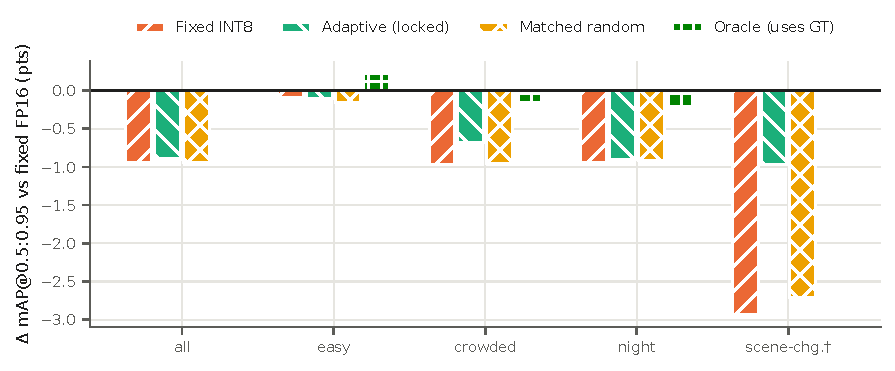
\includegraphics[width=\textwidth]{slices}
% ALT: see figs/alt_text.json ("slices")
\caption{Per-slice mAP@0.5:0.95 difference to fixed FP16 (zero line) on test. The controller follows fixed INT8 and
matched random on every natural slice. Its advantage on the scene-change slice comes from synthetic splices that its own cue detects by construction.}
\label{fig:slices}
\end{figure}

% ============================================================================================
\section{Threats to Validity}\label{sec:threats}
\emph{Scope.} We test one detector (YOLO11s, COCO weights, no fine-tuning), one GPU (Tesla T4) and one dataset. Absolute mAP is low
because of domain shift; our claims are about the relative behaviour of precision policies. We did not run the planned aerial (VisDrone~\cite{visdrone})
or embedded-GPU experiments, did not evaluate INT4, and did not evaluate the hardware-contention term.
\emph{Sample size.} \TestClips{} test and \CalibClips{} calibration clips give wide clip-level intervals. Larger calibration sets might
stabilise the per-condition INT8 gaps, which our diagnosis would predict.
\emph{Data.} Both splits are drawn from the BDD100K tracking validation set (disjoint clips). Labels are at 5\,fps, so motion
cues are coarse. Scene changes are synthetic.
\emph{Engine drift.} Engines rebuilt in the final session differ from earlier builds by up to \DriftINTeight{} points (INT8)
on calibration. All reported numbers use one consistent build.
\emph{Measurement.} Energy is GPU board energy only. Live energy was measured on a two-clip subset on which the controller chose INT8
for every frame. Clocks cannot be locked on a cloud GPU; repeats were interleaved to limit drift.
\emph{Post-hoc changes.} The primary energy metric ($E_\text{total}$ instead of $E_\text{dyn}$) and the evaluation of H3 and H4 were
revised after the test results were seen. Both versions are reported, and nothing was re-tuned or re-run.

% ============================================================================================
\section{Conclusion}
A per-frame oracle shows that a COCO-pretrained YOLO11s could run INT8 on a majority of BDD100K frames without losing FP16 accuracy.
A training-free controller built on motion, clutter, detection count and confidence, and scene-change cues does not realise this.
Once calibrated and locked, it behaves like fixed INT8 and like random switching with the same precision mix, and its cues and second resident
engine cost more energy than fixed INT8. The reason is that INT8 sensitivity per scene condition did not transfer between disjoint clip sets.
Two lessons follow for adaptive-inference work. First, claims should be tested against a matched-random baseline and an oracle, not only against fixed
configurations. Second, signals closer to the detector's own error, such as confidence and uncertainty, and larger calibration sets are more promising than
generic image statistics. All results, configuration hashes and generation scripts are available in the project repository \TODO{repository URL or ``upon request''}.

\paragraph{Licences.} The Ultralytics software and pretrained weights are AGPL-3.0~\cite{ultralytics}, and our code is released
under the same licence. BDD100K is used under its licence for research purposes; no dataset images are reproduced in this paper.
\VERIFY{final licence wording against the BDD100K licence page}

\begin{thebibliography}{10}
\providecommand{\doi}[1]{\url{https://doi.org/#1}}

\bibitem{approxdet2020}
Xu, R., Zhang, C., Wang, P., Lee, J., Mitra, S., Chaterji, S., Li, Y., Bagchi, S.:
ApproxDet: content and contention-aware approximate object detection for mobiles.
In: Proceedings of the 18th ACM Conference on Embedded Networked Sensor Systems (SenSys) (2020).
\doi{10.1145/3384419.3431159}

\bibitem{adascale2019}
Chin, T.-W., Ding, R., Marculescu, D.:
AdaScale: towards real-time video object detection using adaptive scaling.
In: Proceedings of Machine Learning and Systems, vol.~1 (MLSys 2019)

\bibitem{bdd100k}
Yu, F., Chen, H., Wang, X., Xian, W., Chen, Y., Liu, F., Madhavan, V., Darrell, T.:
BDD100K: a diverse driving dataset for heterogeneous multitask learning.
In: Proceedings of the IEEE/CVF Conference on Computer Vision and Pattern Recognition (CVPR), pp. 2636--2645 (2020)

\bibitem{chameleon2018}
Jiang, J., Ananthanarayanan, G., Bodik, P., Sen, S., Stoica, I.:
Chameleon: scalable adaptation of video analytics.
In: Proceedings of ACM SIGCOMM (2018). \doi{10.1145/3230543.3230574}

\bibitem{coco}
Lin, T.-Y., Maire, M., Belongie, S., Hays, J., Perona, P., Ramanan, D., Doll\'ar, P., Zitnick, C.L.:
Microsoft COCO: common objects in context.
In: Fleet, D., et al. (eds.) ECCV 2014, Part V. LNCS, vol.~8693, pp. 740--755. Springer, Cham (2014)

\bibitem{jacob2018}
Jacob, B., Kligys, S., Chen, B., Zhu, M., Tang, M., Howard, A., Adam, H., Kalenichenko, D.:
Quantization and training of neural networks for efficient integer-arithmetic-only inference.
In: Proceedings of the IEEE Conference on Computer Vision and Pattern Recognition (CVPR), pp. 2704--2713 (2018).
\doi{10.1109/CVPR.2018.00286}

\bibitem{liu2022}
Liu, Z., Wang, Y., Han, K., Ma, S., Gao, W.:
Instance-aware dynamic neural network quantization.
In: Proceedings of the IEEE/CVF Conference on Computer Vision and Pattern Recognition (CVPR), pp. 12424--12433 (2022)

\bibitem{nagel2021}
Nagel, M., Fournarakis, M., Amjad, R.A., Bondarenko, Y., van Baalen, M., Blankevoort, T.:
A white paper on neural network quantization. arXiv:2106.08295 (2021)

\bibitem{ultralytics}
Jocher, G., Qiu, J.: Ultralytics YOLO11, version 11.0.0. \url{https://github.com/ultralytics/ultralytics} (2024). AGPL-3.0

\bibitem{visdrone}
Zhu, P., Wen, L., Du, D., Bian, X., Fan, H., Hu, Q., Ling, H.:
Detection and tracking meet drones challenge.
IEEE Trans. Pattern Anal. Mach. Intell. \textbf{44}(11), 7380--7399 (2022). \doi{10.1109/TPAMI.2021.3119563}

\end{thebibliography}
\end{document}
